% !TeX spellcheck = en_GB
\section{Wednesday, \SI{21}{\dec}}
Observed precipitation at the Haukelister measurement site started in the morning and last almost continuesly through the event. The precipitation amount was moderately and as described in \Cref{sec:largeScale} was Norway located within a cold air section. 

%%%%%%%%%%%%%%%%%%%%%%%%%%%%%%%%%%%%%%%%%%%%%%%%%%%%%%%%%%%%%%%%%%%%%%%%%%
%%%%%%%%% vertical obs %%%%%%%%%%%%%%
\subsection{Vertical snowfall observations}
% %%% image SWC SWP %%%%%%%%%%%%%%%%%%%%%%%%%%%%%%%%%%%%%
\begin{figure}[h]
	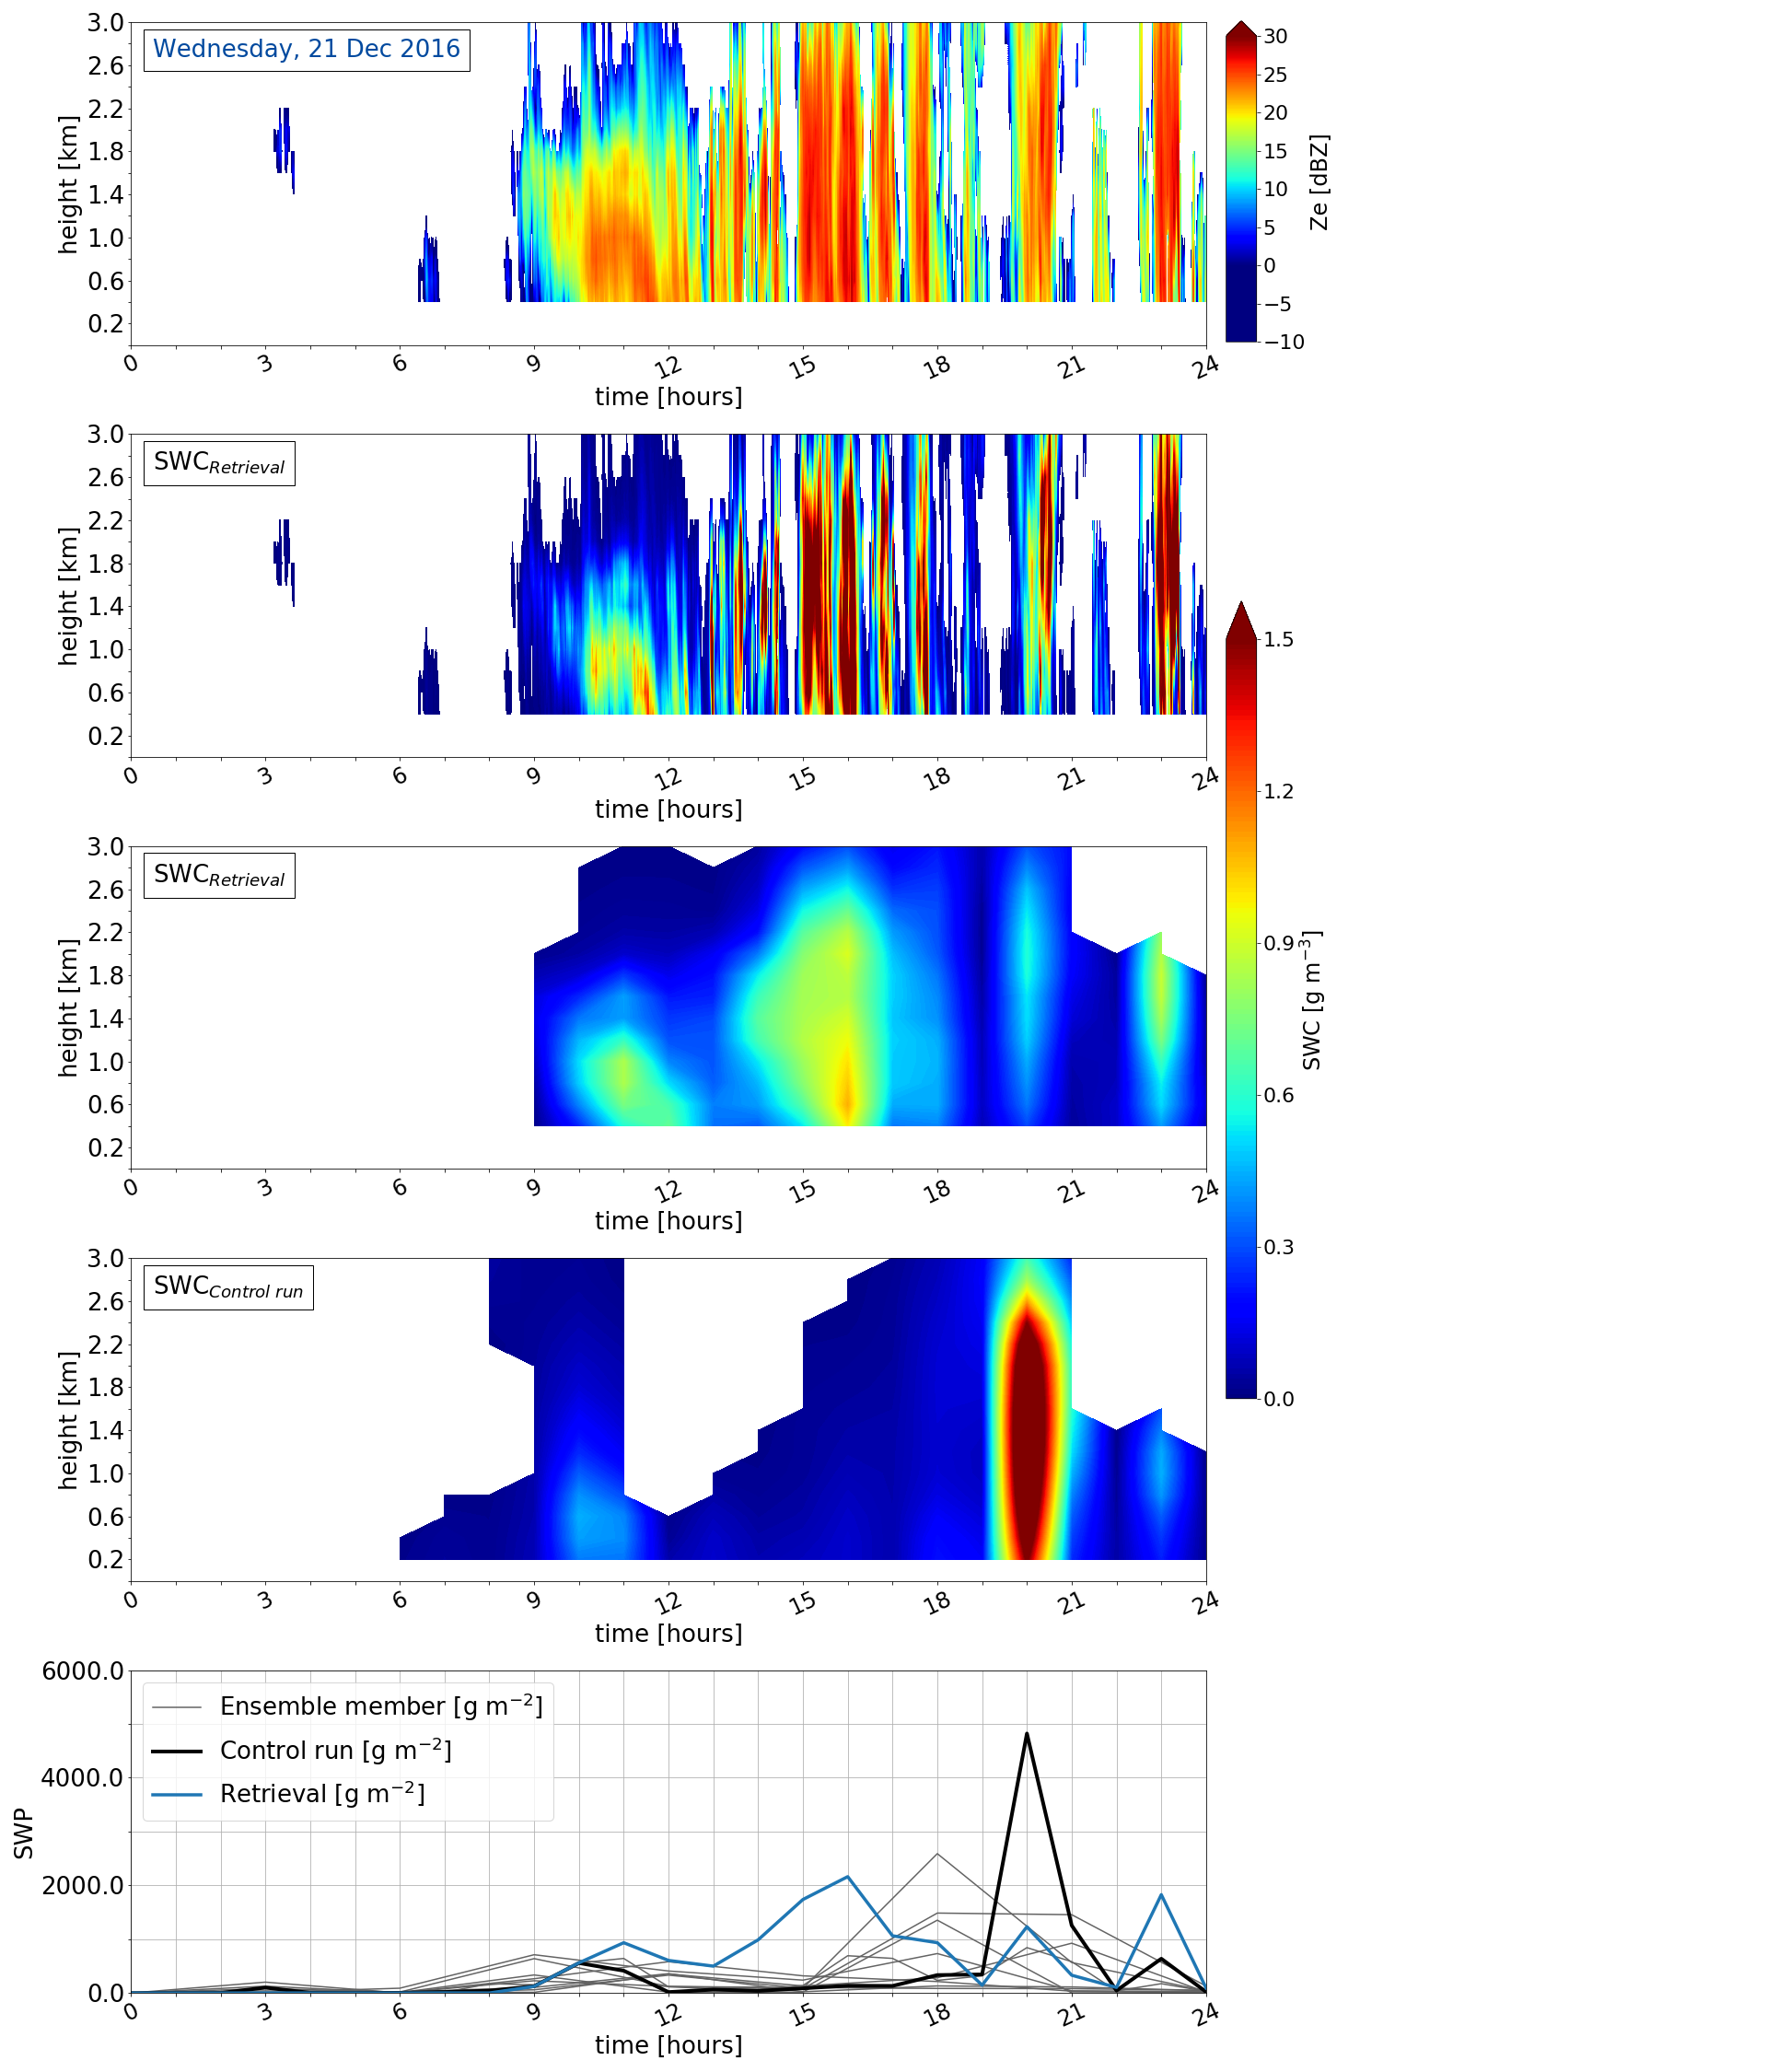
\includegraphics[trim={0.5cm 0.5cm 17.5cm .5cm},clip,width=\textwidth]{./fig_SWC/20161221}
	\caption{Wednesday, \SI{21}{\dec}}\label{fig:SWC21}
\end{figure}
%%%%%%%%%%%%%%%%%%%%%%%%%%%%%%%%%%%%%%%%%%%%%%%%%%%%%%%%%%%%%%%%%%%%%%%%%%
The vertical observations from the MRR and the results of the snowfall retrieval are presented in the three upper panels of \Cref{fig:SWC21}. The first panel shows the transformed radar reflectivity in [\SI{}{\decibel Z}]. Between \SIlist{9;13}{\UTC} was a convective storm observed which afterwards turned into a 'pulsing' with a change of higher and lower reflectivities. 
\\
After applying the forward model (\Cref{sec:forward_model}) the snow water content of the \SI{21}{\dec} is shown. The structure of the convective storm can still be seen, with high values between \SIlist{10;13}{\UTC}. After the pass of the convective storm high reflectivity values up to \SI{25}{\decibel Z} are on and off observed. That follows high snow water content higher than \SI{1.5}{\SWC}. \\
Taking the third panel in \Cref{fig:SWC21} into account, which shows the hourly averaged SWC from the optimal estimation retrieval, one maximum snow water content occurs at \SI{11}{\UTC}, with values up to \SI{0.9}{\SWC}. Associated with the pulsing afterwards is the days SWC maximum of \SI{1.08}{\SWC} monitored at \SI{16}{\UTC} (compare \Cref{tab:max_val}). 
\\
The ensemble mean of all ten ensemble members of MEPS, averaged over \SI{200}{\metre} layers is shown in the third panel. It shows, that the numerical forecast model captures the the convective part of the storm, much weaker but around the same time as observed from the MRR. The high water content around \SI{16}{\UTC} is not observable at all. But MEPS forecasts the pulse at \SI{20}{\UTC} with a maximum of \SI{1.24}{\SWC}.
\\
It shows from the SWP image in \Cref{fig:SWC21}, lower panel that the control run of MEPS (black line) dominates. Most of the other ensemble members (grey line) prognoses the snowfall amount one hour earlier. The blue, dashed line, indicating the ensemble mean SWP shows the weakening of the snowfall amount when taking the average. By comparing the orange line (SWP from the retrieval) and the blue, dashed line it shows, that mean value of MEPS gets closer to the observed one, \SIlist{2833; 2162}{\SWP} respectively.
\\
\textcolor{red}{DISCUSSION! Why does MEPS not catch that peak at \SI{16}{\UTC}? Maybe because it is too close to the convective storm. Also, Why is the control so high compared to the perturbed members?}
%
\newline \noindent
The vertical temperature profile performed with MEPS in \Cref{fig:meps_sound_20} and \ref{fig:meps_sound_21}, shows that an initialisation \SI{36}{\hour} prior to the event would give a cloud with height up to \SI{3}{\km}, as observed in \Cref{fig:SWC21} first panel. An initialisation closer to the occurrence of the storm shows, that MEPS underestimates the intensity and height of the storm (\Cref{fig:meps_sound_21}).
%
%%% image sounding MEPS %%%%%%%%%%%%%%%%%%%%%%%%%%%%%%%%%%%%%
% !TeX spellcheck = en_GB
\begin{figure}
	\centering
	\begin{subfigure}[b]{0.49\textwidth}
		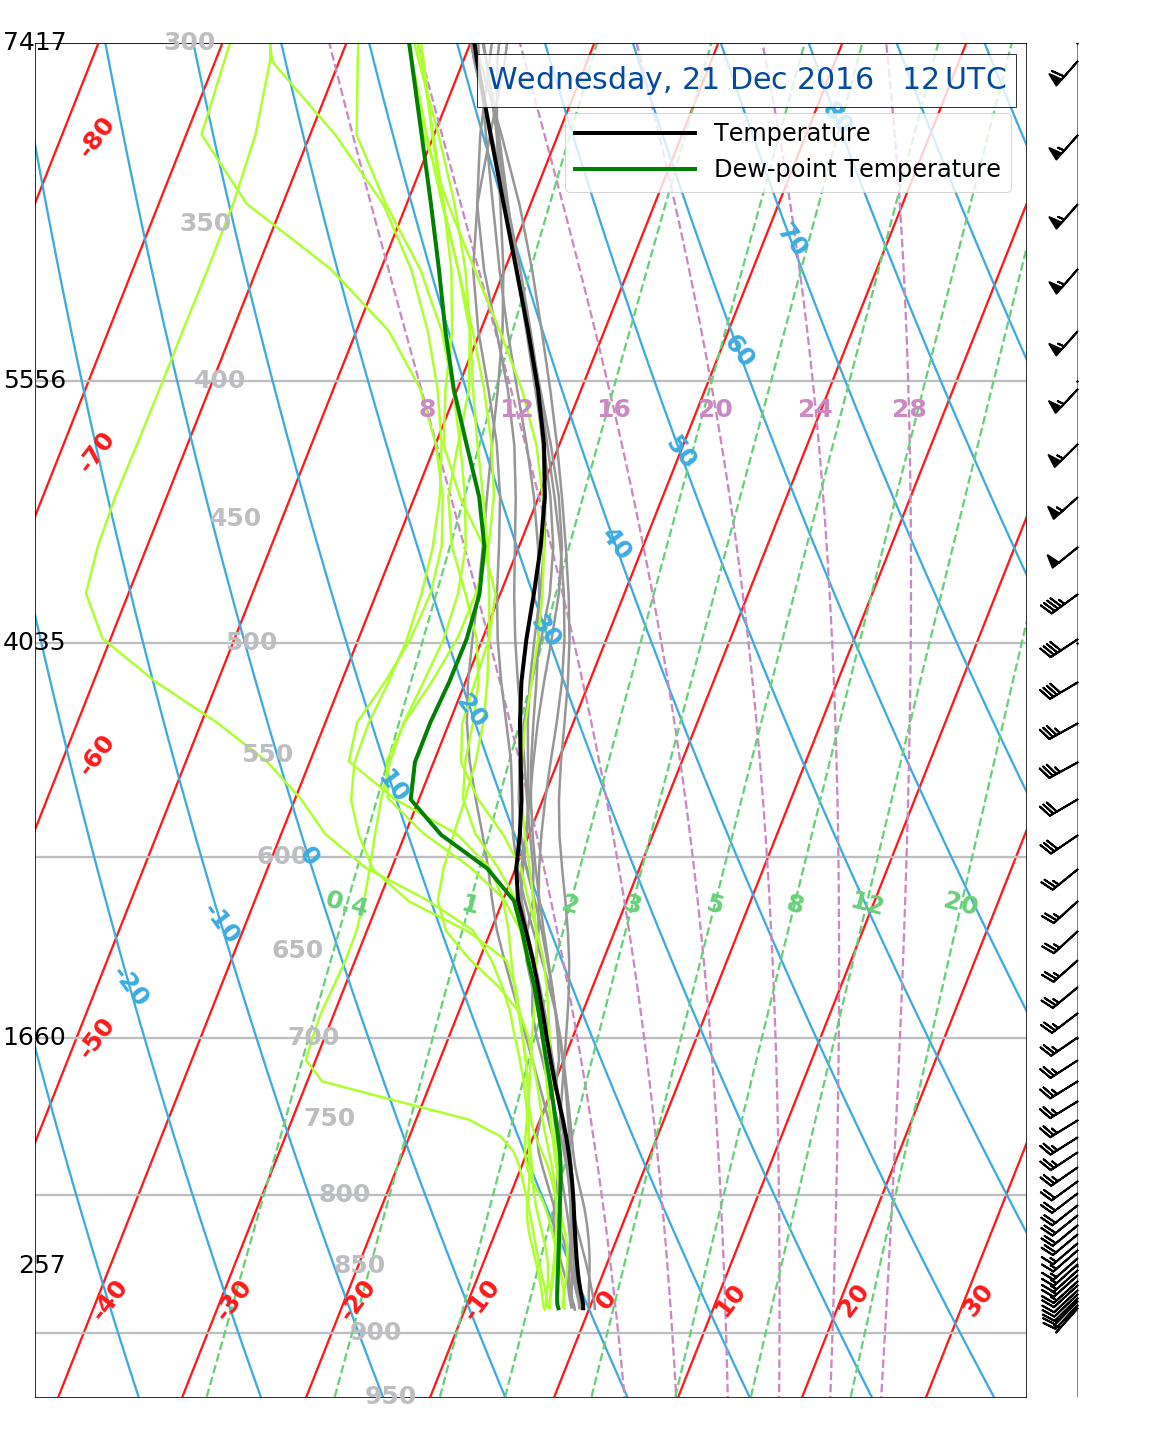
\includegraphics[width=\textwidth]{./fig_Sounding/20161220_36}
		\caption{}\label{fig:meps_sound_20}
	\end{subfigure}
	\begin{subfigure}[b]{0.49\textwidth}
		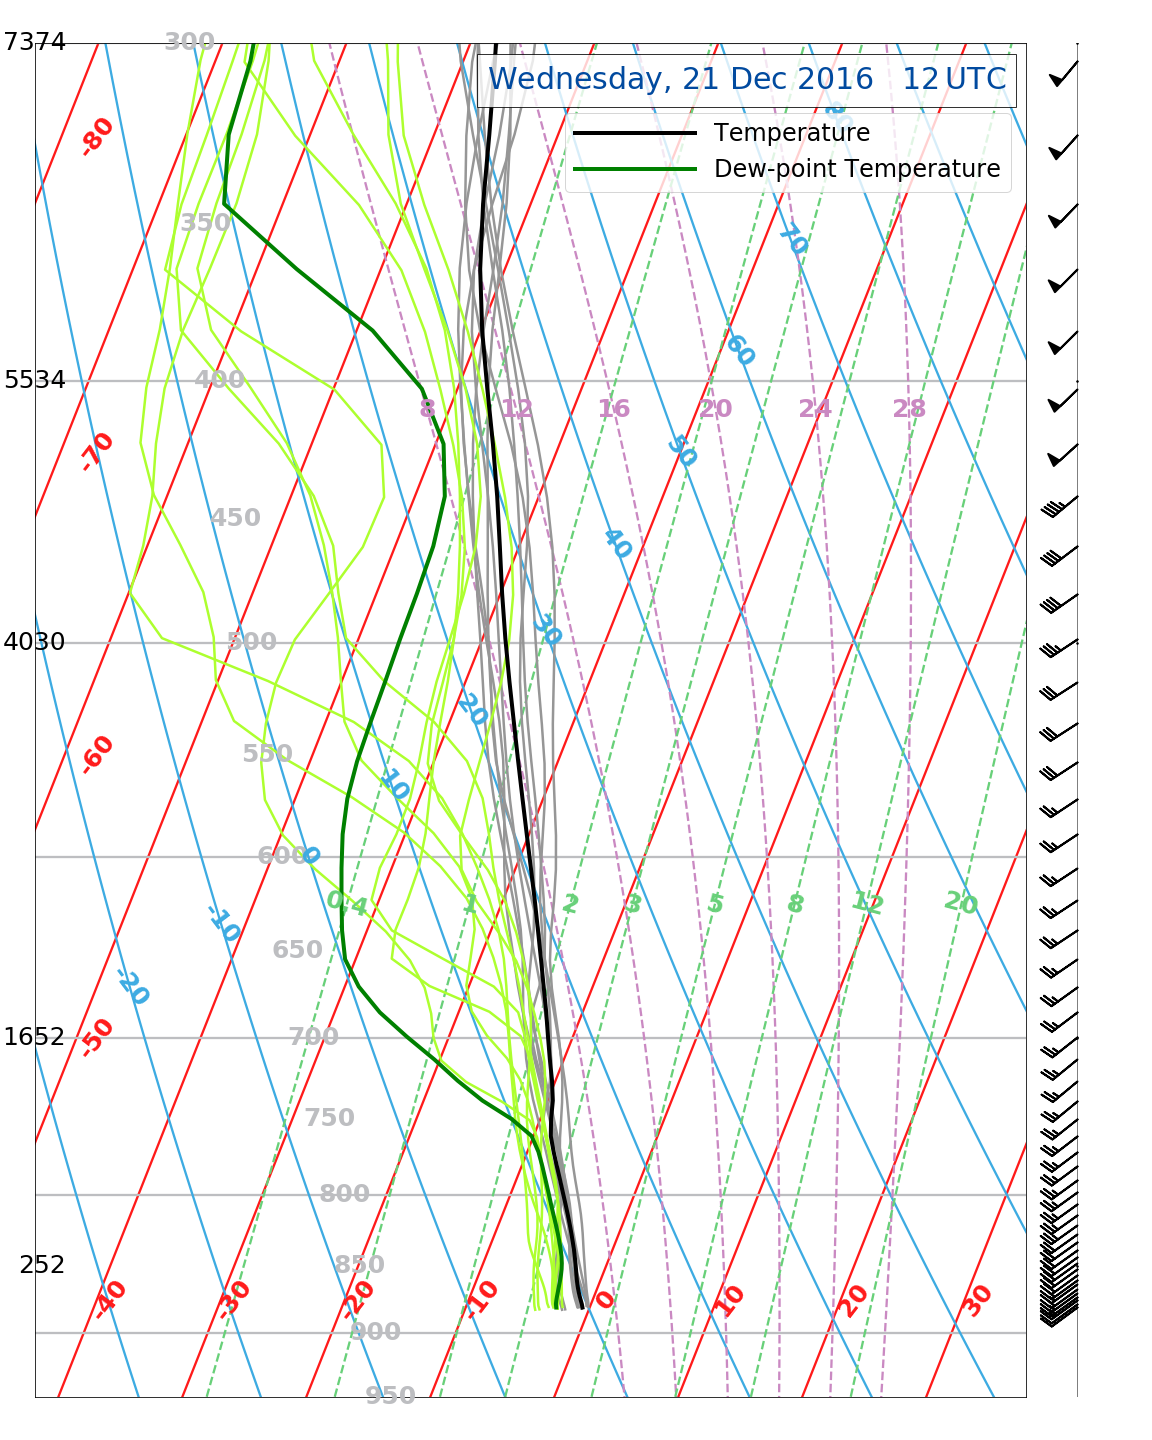
\includegraphics[width=\textwidth]{./fig_Sounding/20161221_12}
		\caption{}\label{fig:meps_sound_21}
	\end{subfigure}
	\caption{Vertical temperature profiles produced with MEPS. \protect{\subref{fig:meps_sound_20}} is initialised: Tuesday, \SI{20}{\dec} \SI{00}{\UTC}. \protect{\subref{fig:meps_sound_21}} is initialised: Wednesday, \SI{21}{\dec} \SI{00}{\UTC}.}
\end{figure}
%%%%%%%%%%%%%%%%%%%%%%%%%%%%%%%%%%%%%%%%%%%%%%%%%%%%%%%%%%%%%%%%%%%%%%%%%%
%
\newline \noindent
The ensemble spread in \Cref{fig:spread21} shows that almost all the members agree, that snowfall is likely to occur around \SIlist{9;12}{\UTC} the spread of the ensemble members is small. The spread increases with forecast time and peaks at \SI{20}{\UTC} with a maximum spread of \SIrange{1.2}{1.3}{\SWC}. 
% 
%%% image ensemble spread %%%%%%%%%%%%%%%%%%%%%%%%%%%%%%%%%%%%%
\begin{figure}[h]
	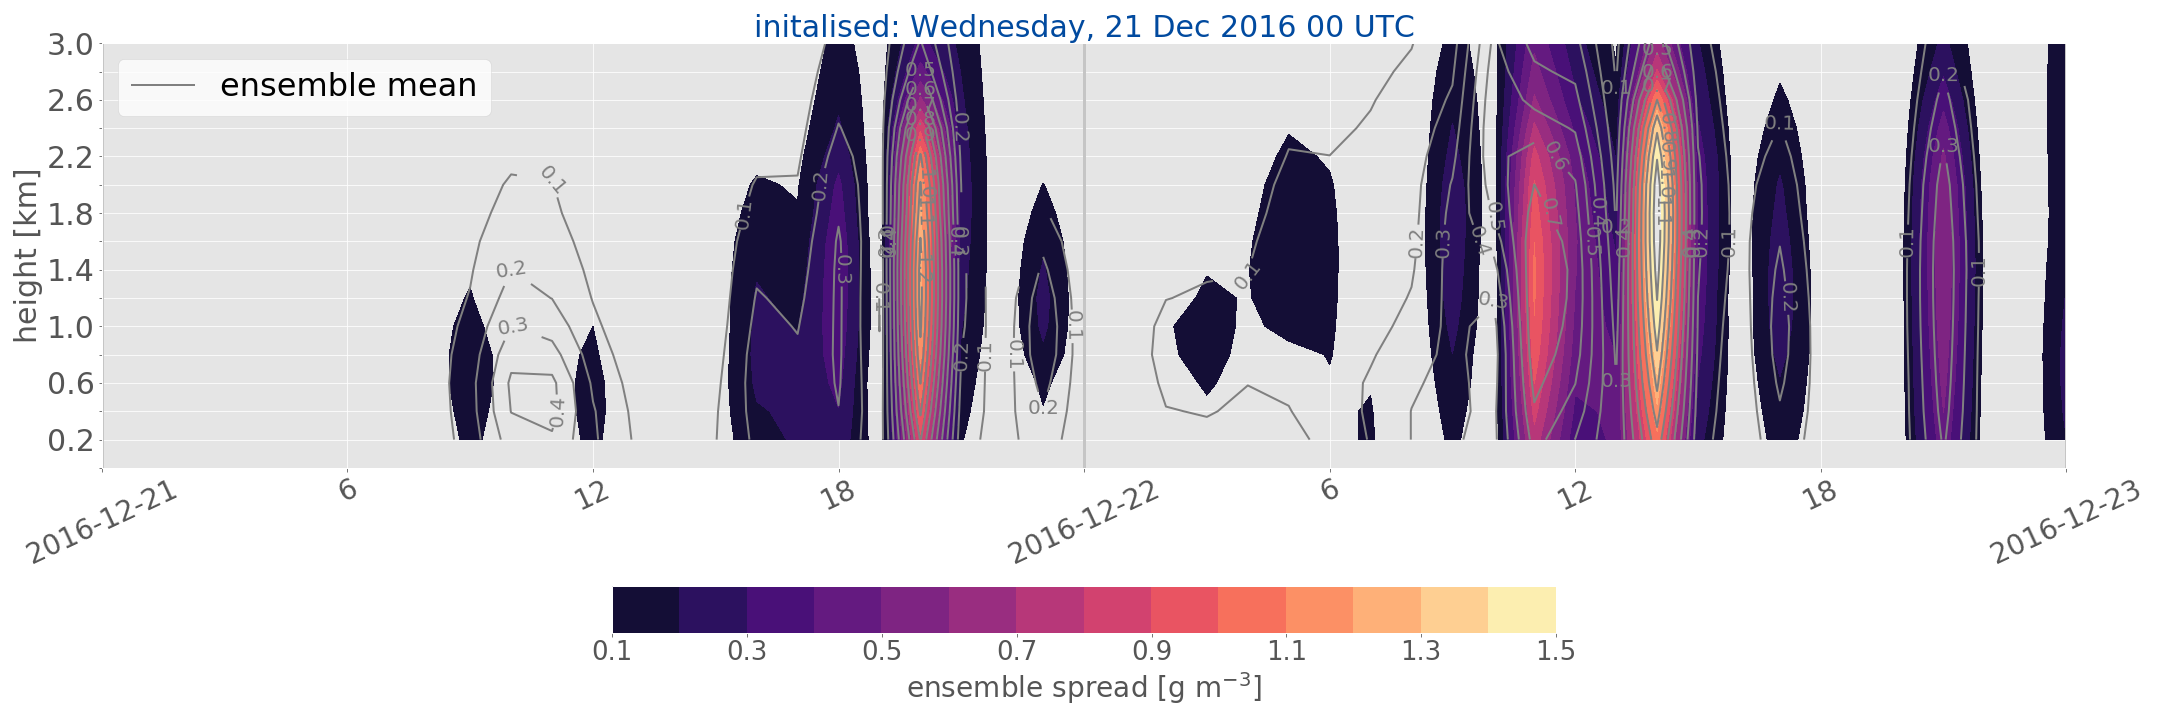
\includegraphics[width=\textwidth]{./fig_ensemble_spread/20161221}
	\caption{Ensemble spread indicated by the colour bar. Lighter colours show higher spread and darker colour very small spread of the ensemble members. Grey lines show the ensemble mean of the ten forecast members.}\label{fig:spread21}
\end{figure}
%%%%%%%%%%%%%%%%%%%%%%%%%%%%%%%%%%%%%%%%%%%%%%%%%%%%%%%%%%%%%%%%%%%%%%%%%%
%
%%%%%%%%%%%%%%%%%%%%%%%%%%%%%%%%%%%%%%%%%%%%%%%%%%%%%%%%%%%%%%%%%%%%%%%%%%
%%%%%%%%% surface obs %%%%%%%%%%%%%%
\subsection{Surface accumulation}
% %%% image surface accumulation %%%%%%%%%%%%%%%%%%%%%%%%%%%%%%%%%%%%%
% \begin{figure}[h]
% 			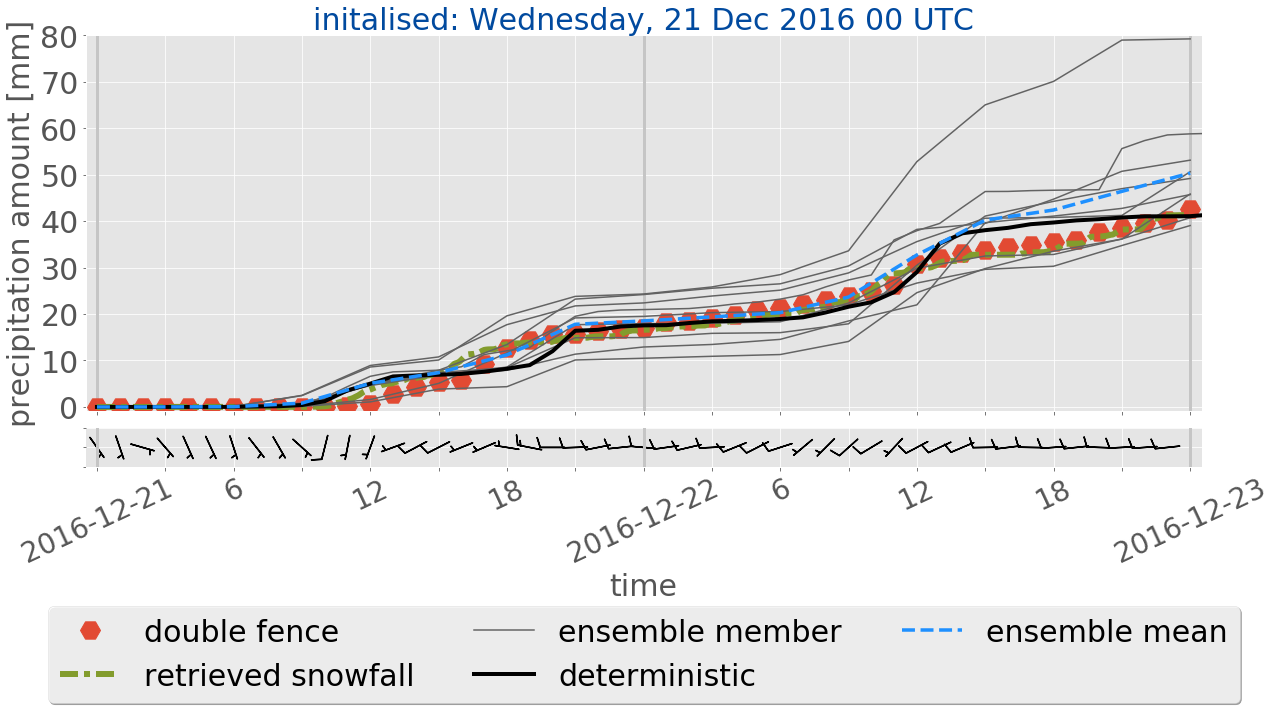
\includegraphics[width=\textwidth]{./fig_sfc_acc/acc_wind_20161221_00}
% 			\caption{}\label{fig:sfc_acc21}
% \end{figure}
% %%%%%%%%%%%%%%%%%%%%%%%%%%%%%%%%%%%%%%%%%%%%%%%%%%%%%%%%%%%%%%%%%%%%%%%%%%
The surface accumulation at the ground showed a good agreement between retrieved snowfall amount, MEPS precipitation amount, and the reference frame of the double fence gauge. Since MEPS had some outlier ensemble members a box-whisker-plot is been provided.
%%% image surface MEPS boxplot %%%%%%%%%%%%%%%%%%%%%%%%%%%%%%%%%%%%%
\begin{figure}[h]
	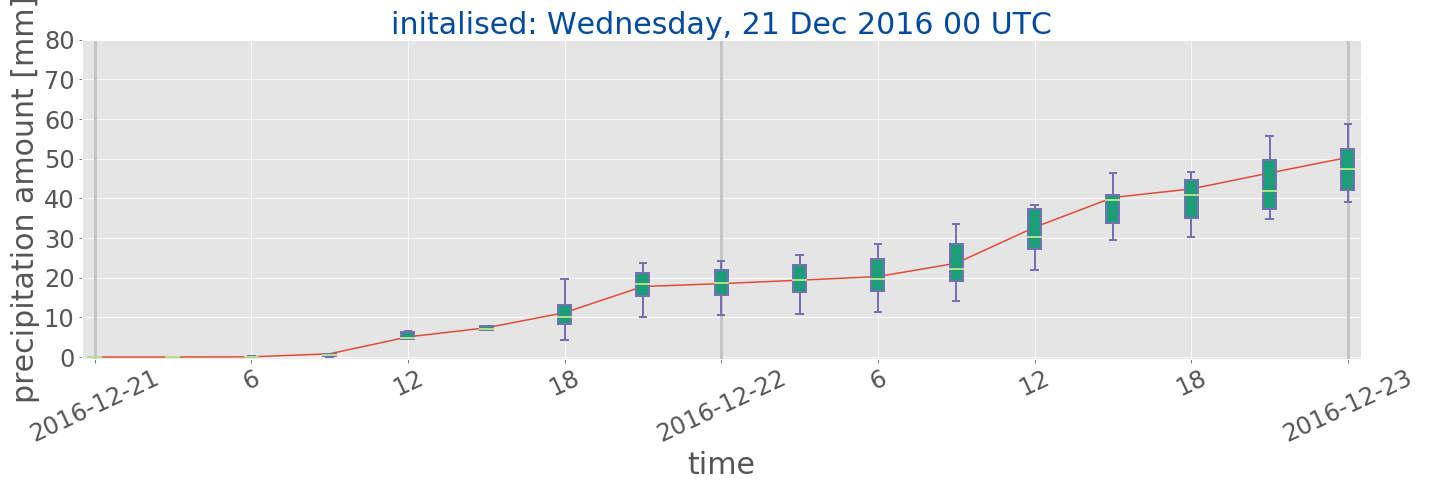
\includegraphics[width=\textwidth]{./fig_boxplot_sfc/20161221_0}
	\caption{Box-whisker-plot of the ten ensemble members of MEPS. Red line indicating the ensemble mean, lower and upper whisker the 25th and 75th percentile, respectively. Light green shows the median of all members and the box represents the middle \SI{50}{\percent} of scores of the precipitation.}\label{fig:boxplt21}
\end{figure}
%%%%%%%%%%%%%%%%%%%%%%%%%%%%%%%%%%%%%%%%%%%%%%%%%%%%%%%%%%%%%%%%%%%%%%%%%%
The box-whisker-plot in \Cref{fig:boxplt21} shows the distribution of the ten ensemble members. In the first \SI{15}{\hour} of the forecast time agree all members well, since the box and whiskers are small. With increasing forecast time, increases the uncertainty. After \SI{30}{\hour} is the ensemble mean slightly higher than the median of the data. In general can the surface forecast be trusted since the values of the ensemble members are well distributed around the mean.
%%% image surface MEPS boxplot %%%%%%%%%%%%%%%%%%%%%%%%%%%%%%%%%%%%%
\begin{figure}[h]
	%	\centering
	\begin{subfigure}[b]{0.84\textwidth}
		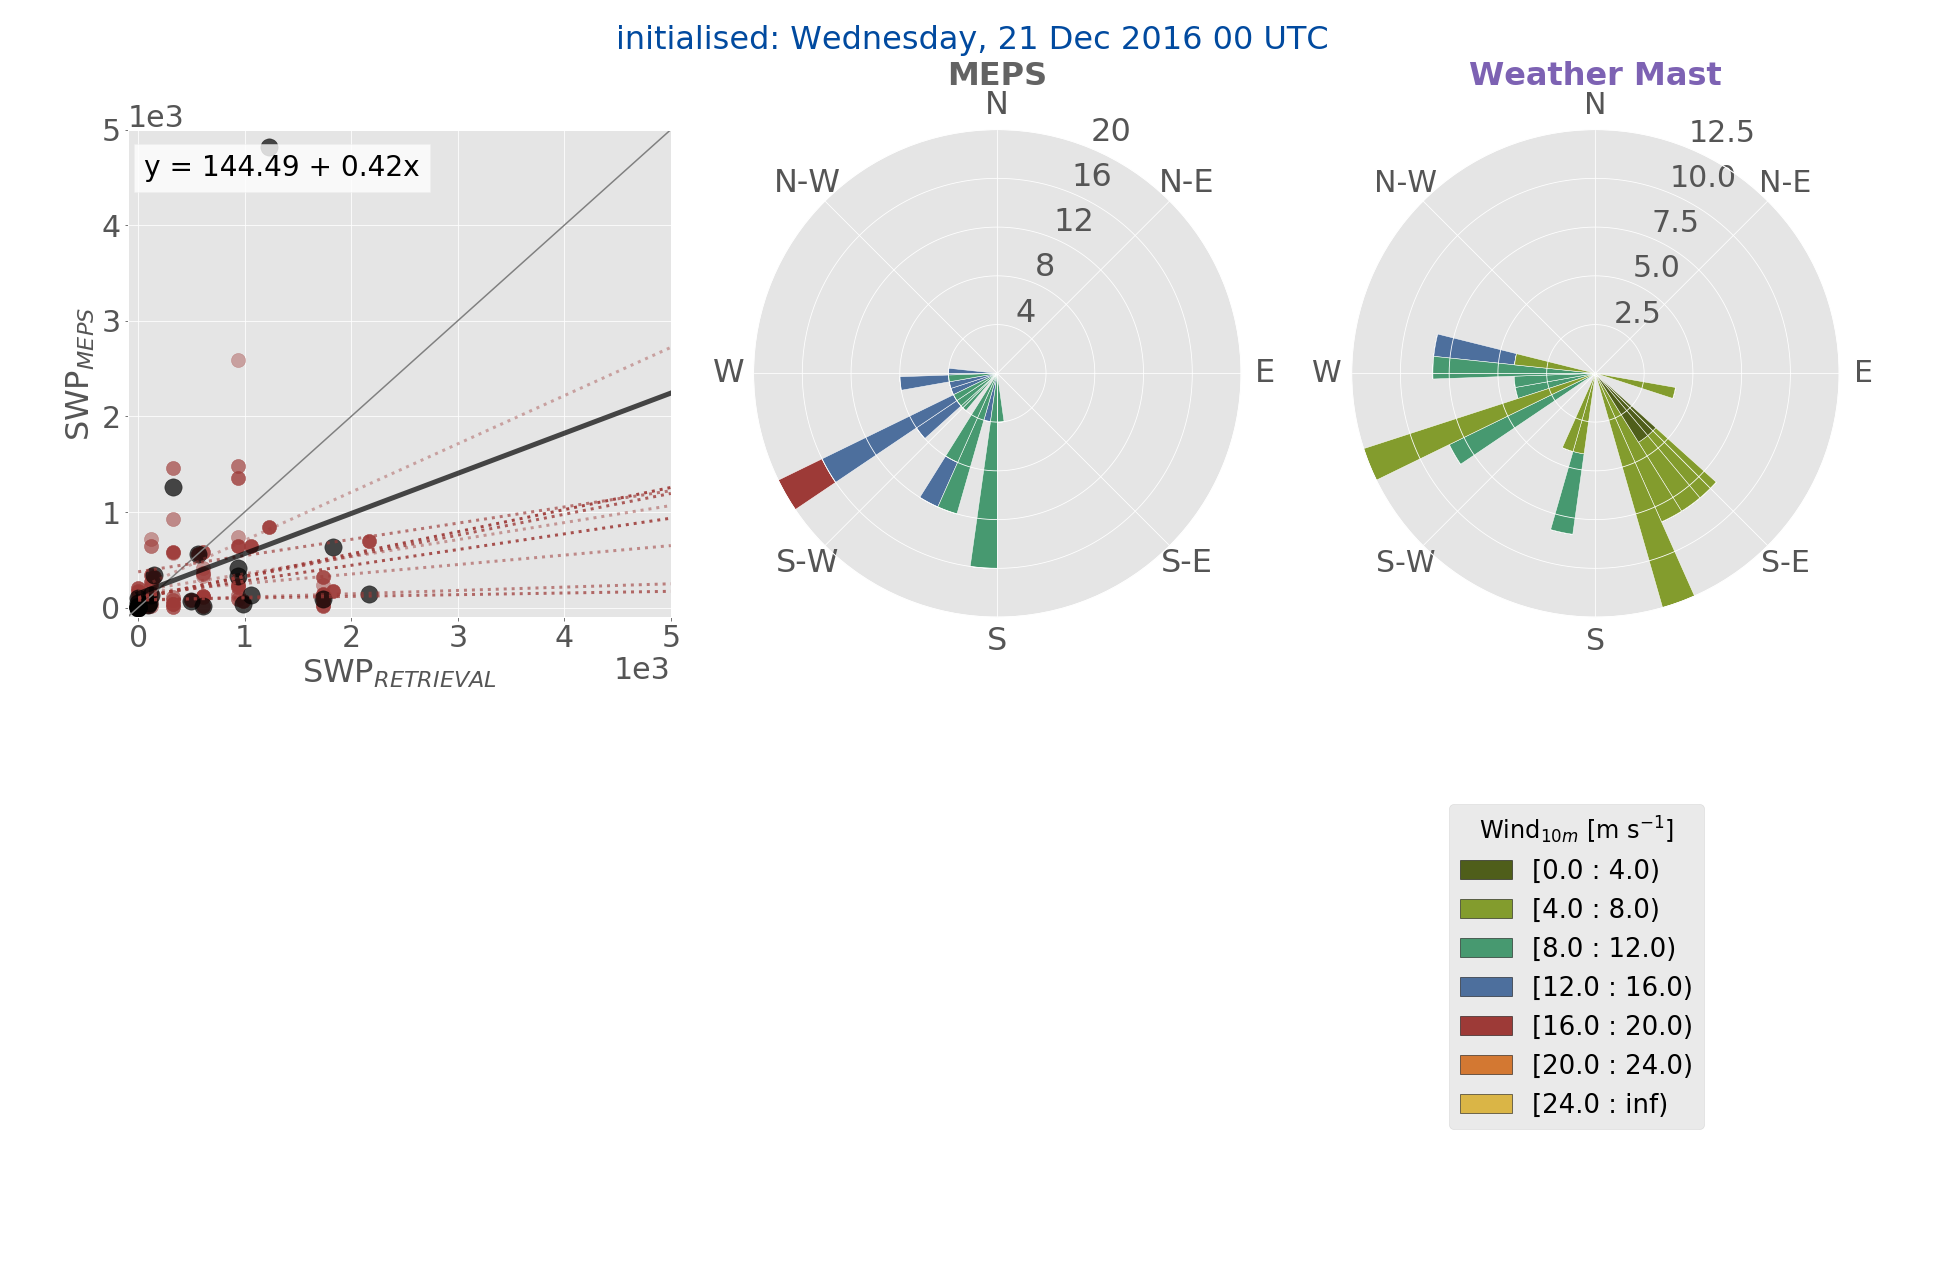
\includegraphics[trim={2.3cm 19.5cm 2.cm .7cm},clip,width=\textwidth]{./fig_windrose/20161221}
	\end{subfigure}
	\begin{subfigure}[b]{0.15\textwidth}
		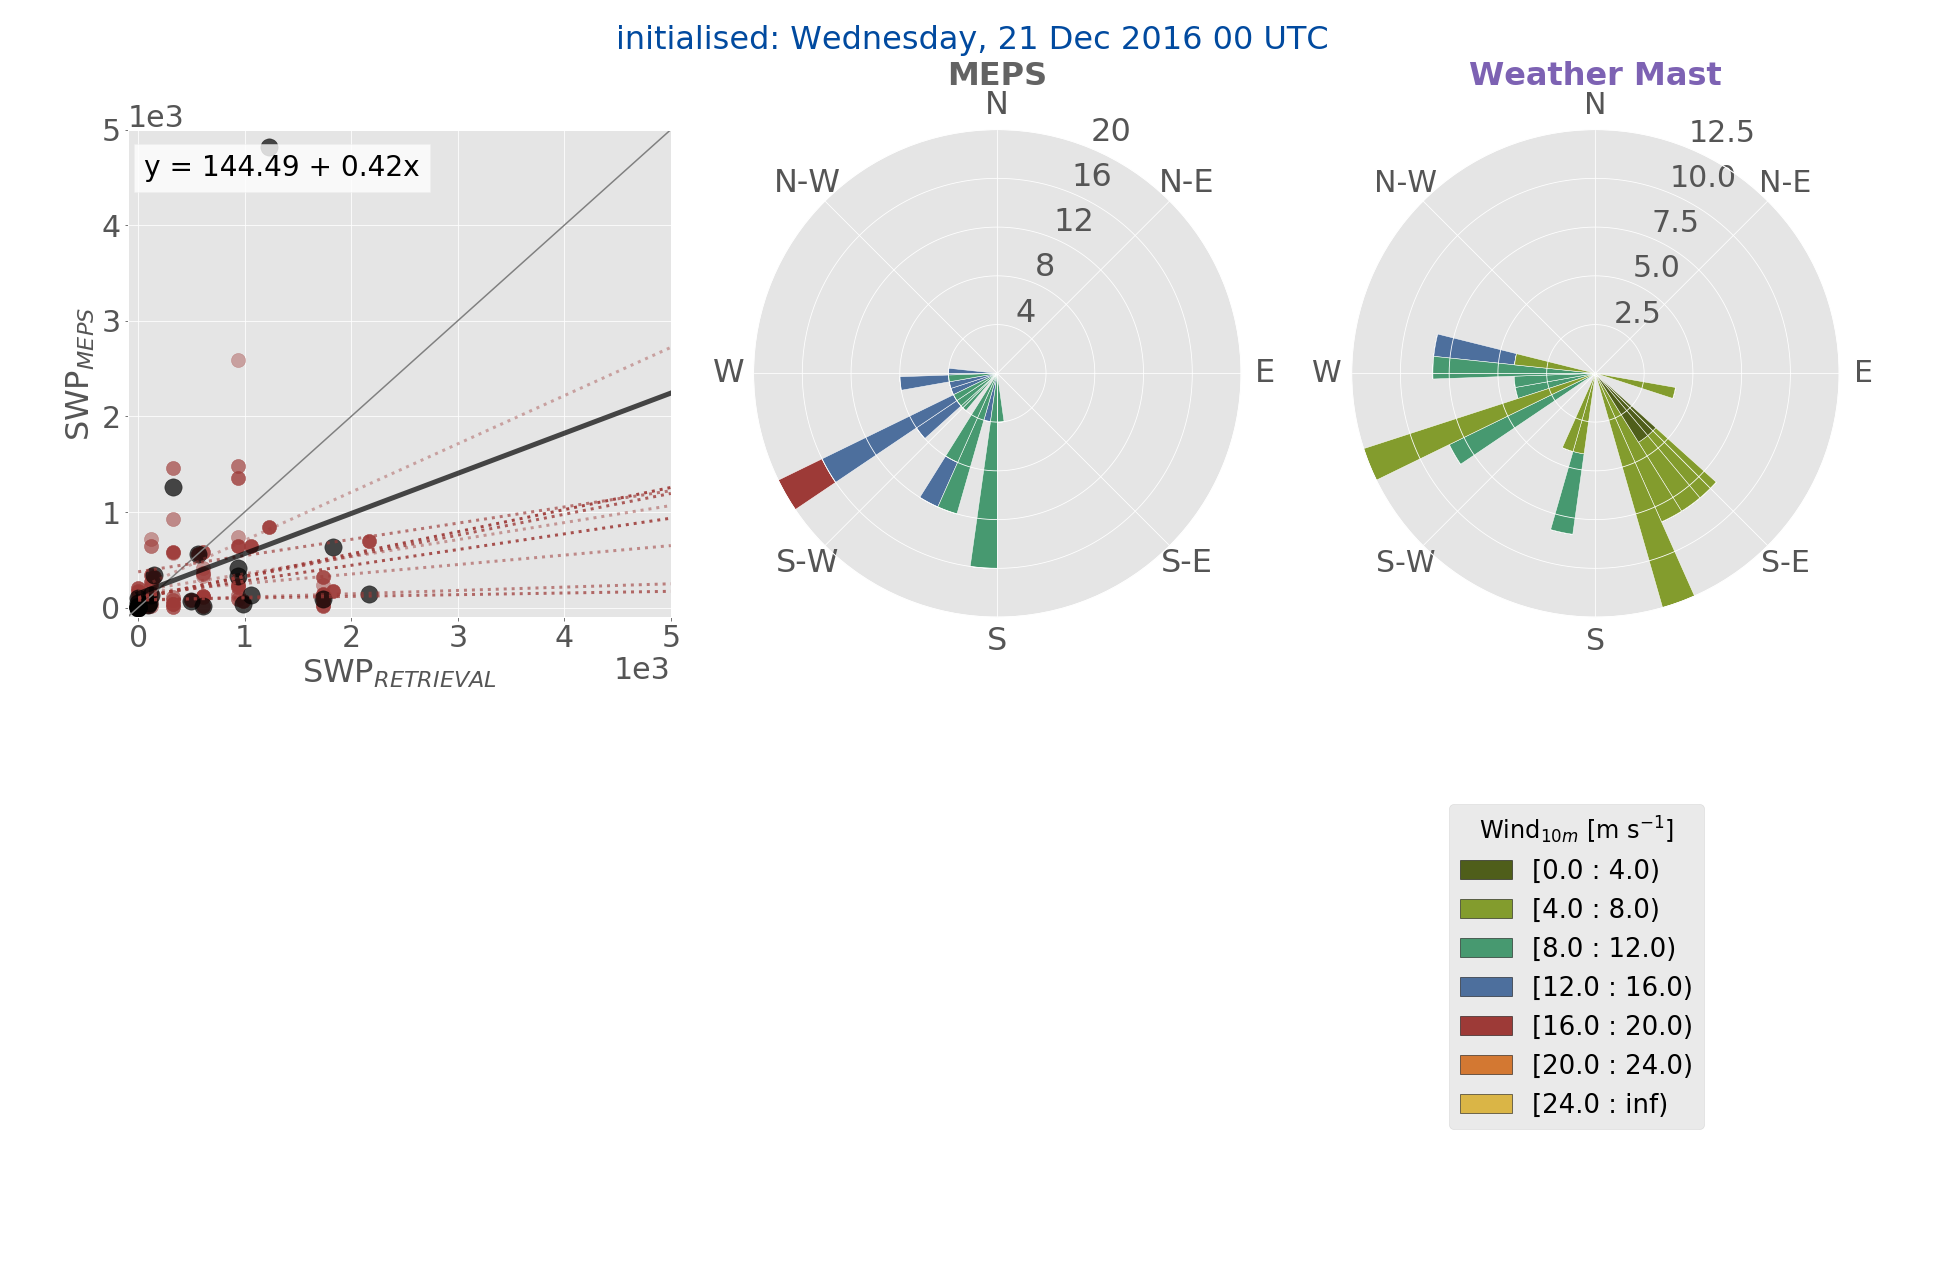
\includegraphics[trim={50.cm 0.cm 8.3cm 28.4cm},clip,width=\textwidth]{./fig_windrose/20161221}
	\end{subfigure}
	\caption{}\label{fig:wind21}
\end{figure}
%%%%%%%%%%%%%%%%%%%%%%%%%%%%%%%%%%%%%%%%%%%%%%%%%%%%%%%%%%%%%%%%%%%%%%%%%%
A relation between the SWP and the surface wind can be shown in \Cref{fig:wind21}. The scatter plot on the left shows, that  the values obtained by the optimal estimation retrieval are stronger than the deterministic prognoses from MEPS, black dots and black line. The nine perturbed ensemble members in red indicate even weaker forecast than actually measured. 
\\
Comparison between the ensemble mean wind and the weather mast show a good agreement, were MEPS observed more often higher values. 
\\
%%%%%%%%%%%%%%%%%%%%%%%%%%%%%%%%%%%%%%%%%%%%%%%%%%%%%%%%%%%%%%%%%%%%%%%%%%
\textcolor{red}{DISCUSSION! The observations from \Cref{fig:SWC21} have shown, that south easterly wind is associated with convective storms. If west wind was observed the MRR reflectivity showed patterns of convection. West wind is one of the main wind directions at Haukeliseter (\Cref{sec:int:dec_obs}) and the event showed always a 'pulsing' pattern when west wind occurred.  }
























